\chapter{Images}

Images are a key part of making the page look more appealing to the reader, however they need to be chosen and placed with some consideration.

\section{Image Placement}

Images should only ever be unit column widths in size, i.e. one/two/three/four/five column widths in size. They should never be extended into the next column, since the word wrapped text in the half column they will occupy will tend to be disjointed and may need hypenation.

The only time an image should extend by a half column is if it is contained in a column that is 1.5 times wider than than the usual column width. 

\section{Image Quality}

When sourcing images to use for a page, an editor should look for large images only. If searching via Google Images online, make sure to filter the image search to large images only. After placing the image on your page, check the \textbf{Links panel} in the palette on the right hand side of the screen (also available by using \shiftkey \cmdkey D).

All images should have an \textbf{Effective PPI} of at least \textbf{150} in the links panel.


\section{Image Colour Space}

\begin{wrapfigure}{r}{5cm}
\vspace{-22pt}
\begin{center}
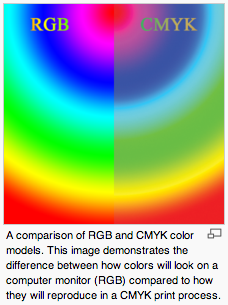
\includegraphics[width=4.8cm]{rgb-cmyk}
\end{center}
\vspace{-50pt}
\end{wrapfigure} 
All images you will encounter on the internet and from a camera will be recorded using the RGB (Red Green Blue), colour space, however printers print using the Cyan Magenta Yellow blacK (CMYK) colour space. This means that we need to convert all of our images into CMYK before we send the paper to the printers. This means that if any images are not easily reproduced in the CMYK colour space (i.e. pictures with large amounts of R, G or B), they can be adjusted before being sent of to print. This can be done using the Felix Droplet (ask Editor for more information).

Please note: Greyscale images do not need to be converted to CMYK, however it is good practise (in order to keep up the habit).

\section{Credits and Captions}


\subsection{Credits}

All images need to be credited. Google Images is not a suitable credit for any image. At the very least, if an image can only be traced back to a blog, the name of the blog can be used as the credit.
Images are credited using the "Photo Credit" paragraph style located in the Felix 2013-14 -> Photo/Image folder in the "Paragraph Styles" panel. Image credits are always placed on the line directly under the image on the right hand side. In some cases when this is not possible the credit can instead be printed in \textbf{white/paper} on a black bar at the bottom of the image.

N.B. When crediting websites, the "https://www" is always omitted. 

\subsection{Captions}

Captions also exist on the line directly under an image. These are left-aligned (never justified) and can fill the space under the picture (up to the credit location). Captions are optional, but credits are mandatory.


